\chapter{La modélisation du carrefour}

% Intro du chapitre : ma modélisation est basée sur OSM donc je décris ce que contient OSM

Le carrefour peut être un espace d'interaction entre piétons et véhicules. Dans le cas où il permet à un piéton de le franchir, la signalisation permet alternativement aux flux des piétons ou des voitures de le traverser en sécurité. Pour une \gls{pcdv}, cette traversée peut être complexe en raison de la variabilité et l'hétérogénéité des configurations, du nombre de voies présentes, et des équipements de contrôle du trafic et d'accessibilité. Dans ce chapitre, nous présentons l'architecture du carrefour du point de vue d'une personne concernée, puis nous analysons au regard des besoins évoqués la manière dont ces données sont représentées dans la base de données \gls{osm}. Enfin, nous proposons une représentation objet de la donnée \gls{osm} que nous appliquons à une modélisation du carrefour orientée sur l'accessibilité.

% Un "état de l'art" à la JLZ pour chaque sous-partie : une vue précise du carrefour, de son infrastructure et des éléments d'accessibilité qui le compose.
% Penser le carrefour du point de vue du piéton sous la forme d'un graphe 

\section{La structure globale du carrefour}

% Pour définir les éléments de mon modèle, j'ai utilisé des méthodo de travail : je suis allé interroger des professionnels, etc. Mentionner le fait d'être allé rencontrer des personnes du CRDV, autres professionnels.

Un carrefour, tel que défini par le dictionnaire Larousse, est un \pquote{lieu où se croisent plusieurs rues ou plusieurs routes, généralement aménagé en vue d'éviter les risques de collision, et parfois d'améliorer le débit}. Une particularité concernant nos travaux est que le carrefour nous intéresse du point de vue du piéton, et notamment du piéton concerné par la déficience visuelle, dont les spécificités doivent être prise en compte dans la définition d'un carrefour tel que nous le concevons. Lors des travaux préliminaires à ce mémoire, nous avons interrogé des personnes concernées et professionnels du \gls{crdv} de Clermont-Ferrand pour établir cette définition. Pour ces dernières, la limite d'un carrefour correspond à l'étendue de ce qu'une personne peut entendre. Bien qu'il existe des travaux de modélisation accoustique\comment{Ajouter une référence} orientés notamment sur la propagation du bruit, cette approche nous semble difficile à généraliser dans un premier temps. Nous avons donc choisi de nous concentrer tout d'abord sur la structure du carrefour du point de vue du piéton, en en proposant une représentation sous forme de graphe, puis en s'intéressant aux élements d'accessibilité spécifiques à la mobilité des \glspl{pcdv}.

\begin{figure}
    \centering
    \resizebox{15cm}{!}{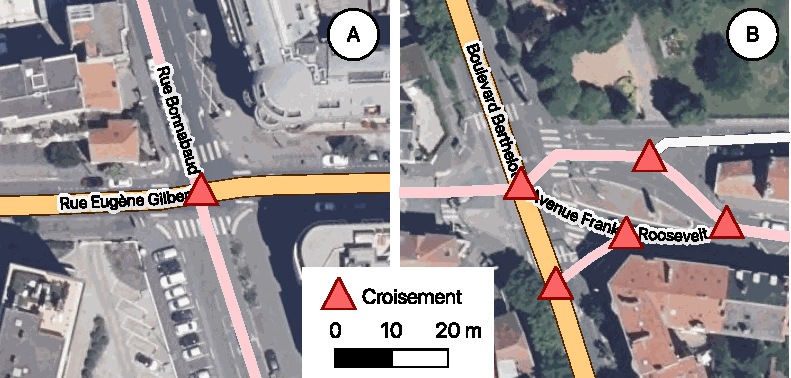
\includegraphics{images/modelisation/mod_simple_complexe.pdf}}
    \caption[La délimitation du carrefour]{Un carrefour peut être difficile à délimiter quand il ne s'agit pas d'un unique croisement. La délimitation du carrefour B dépend de la définition que l'on souhaite prendre du carrefour, et peut être en réalité composé de plusieurs sous-carrefours. Sources : Orthophotographie CRAIG, Contributeurs OpenStreetMap.}
    \label{fig:modelisation_simplecomplexe}
\end{figure}

% Structure en branches
% On se place du point de vue du piéton, ce sont les trottoirs qui comptent.

\subsection{Le graphe du carrefour du point de vue d'un piéton}

Pour modéliser le carrefour du point de vue d'un piéton, nous avons choisi de nous reposer sur une approche graphe afin de le définir et de le délimiter dans un réseau routier. Les définitions suivantes en définissent la structure :

\begin{definition}
    On appelle \textbf{couverture} d'un graphe $G_0 = (V_0,E_0)$ connexe et plongé dans le plan un ensemble de sous-graphes connexes $\mathcal{G_0}$ tels que:
    \begin{itemize}
        \item Si $G_1=(V_1, E_1) \in \mathcal{G_0}$ et $G_2=(V_2, E_2) \in \mathcal{G_p}$, alors $E_1 \cap E_2 = \emptyset$
        \item $\forall e \in E_p$, $\exists!~G_1=(V_1, E_1) \in \mathcal{G_p}$ tel que $e \in E_1$
    \end{itemize}
    
    Dans la suite, on appelle $\mathcal{G}_p$ une couverture du graphe piéton, et $\mathcal{G}_r$ une couverture du graphe routier.
    
    Dans la suite, on dira que deux sous-graphes sont \textbf{connectés} s'ils partagent au moins un sommet en commun.
\end{definition}

\begin{definition}
    On défini un \textbf{graphe multimodal} comme un graphe $G = (V,E)$ connexe et plongé dans le plan et muni d'une couverture $\{G_r=(V_r, E_r), G_p = (V_p, E_p)\}$ composée d'un \textbf{graphe routier} $G_r$ et d'un \textbf{graphe piéton} $G_p$.

    Remarque: l'intersection entre $V_r$ et $V_p$ peut ne pas être vide.

    Dans la suite, on note $G = (V,E)$ un graphe multimodal sur lequel on défini les autres ensembles et propriétés.
\end{definition}

\begin{definition}
    Soient $G_1=(V_1, E_1)$ et $G_2=(V_2, E_2)$ deux sous-graphes de $G=(V, E)$.
    
    On appelle \textbf{fonction d'association} $f: E_1 \rightarrow E_2$ toute fonction qui à chaque arête de $G_1$ associe une arête de $G_2$.
\end{definition}

\begin{definition}
    Alors on appelle \textbf{trottoir} tout $G_t = (V_t, E_t)\in \mathcal{G}_p$ sous-graphe du graphe piéton muni d'une fonction d'association $f_t: G_t \rightarrow G_r$ projetant les arêtes de $G_t$ dans le graphe routier. Cette fonction $f_t$ est appelée \textbf{fonction d'adjacence} du trottoir $G_t$.

    On note $\mathcal{G}_t$ l'ensemble des trottoirs.
\end{definition}

\begin{definition}
    Étant donné une couverture $\mathcal{G}_p$ d'un graphe piéton $G_p$, un ensemble de fonctions d'adjacence est dit \textbf{un ensemble de trottoirs couvrants} s'il n'existe pas de sommet $v \in G_p$ appartenant à plus d'un trottoir.

    Exemple: couverture d'un graphe piéton qui n'est pas un ensemble de trottoirs couvrants (voir Figure \ref{fig:mod_ex_trottoirs_couvrants}).
\end{definition}

\begin{figure}
    \centering
    
\includegraphics{images/placeholder.jpg}
    \caption{Ces deux trottoirs ne sont pas couvrants car ils possèdent un noeud en commun.}
    \label{fig:mod_ex_trottoirs_couvrants}
\end{figure}

\begin{definition}
    On appelle \textbf{chemin} un graphe $G_{ch} = (V_{ch}, E_{ch})$ tel que $V_{ch}=\{p_1,p_2,\dots,p_n\}$ et $E_{ch}=\{\{p_1,p_2\},\{p_2,p_3\},\dots,\{p_{n-1},p_n\}\}$.
\end{definition}

\begin{definition}
    Un \textbf{passage piéton} $G_{pp} = (V_{pp}, E_{pp}) \in \mathcal{G}_p$ est un chemin $(p_1, p_2,\dots, p_n)$ tel que:

    \begin{itemize}
        \item $p_2, p_3, \dots, p_{n-1}$ sont inclus dans le graphe routier
        \item $p_2, p_3, \dots, p_{n-1}$ n'appartiennent pas à un trottoir
        \item $p_1$ et $p_n$ appartiennent chacun à un trottoir
    \end{itemize}
\end{definition}

\begin{definition}
    Une couverture $\mathcal{G}_r$ d'un réseau routier est dite \textbf{couverture routière complète} si et seulement si elle est composée d'une union disjointe de \textbf{coeurs de carrefours} $\mathcal{G}_c \subset \mathcal{G}_r$ et de \textbf{branches} $\mathcal{G}_b \subset \mathcal{G}_r$ tels que:

    \begin{itemize}
        \item $\mathcal{G}_c \neq \emptyset$ 
        \item Deux coeurs de carrefour ne sont pas connectés
        \item Chaque branche est connectée à un ou deux coeurs de carrefour
        \item Un coeur de carrefour est au minimum connecté à deux branches distinctes
    \end{itemize}

    Exemples:
    \begin{itemize}
        \item Une couverture routière qui n'est pas complète (voir Figure \ref{fig:mod_ex_couverture_routiere_incomplete})
        \item Une couverture routière de carrefour (voire Figure \ref{fig:mod_ex_couverture_routiere_carrefour})
        \item Une couverture routière à plusieurs carrefours, dites de quartier (voire Figure \ref{fig:mod_ex_couverture_routiere_quartier})
    \end{itemize}
\end{definition}

\begin{figure}
    \centering
    
\includegraphics{images/placeholder.jpg}
    \caption{Cette couverture routière est incomplète car \todo{}.}
    \label{fig:mod_ex_couverture_routiere_incomplete}
\end{figure}

\begin{figure}
    \centering
    
\includegraphics{images/placeholder.jpg}
    \caption{Cette couverture de carrefour montre \todo{}.}
    \label{fig:mod_ex_couverture_routiere_carrefour}
\end{figure}

\begin{figure}
    \centering
    
\includegraphics{images/placeholder.jpg}
    \caption{Une couverture de quartier comprend plusieurs carrefours.}
    \label{fig:mod_ex_couverture_routiere_quartier}
\end{figure}

\begin{definition}
    Une couverture $\mathcal{G}_p$ d'un réseau piéton est dite \textbf{couverture piétonne complète} si et seulement si elle est composée d'une union disjointe de trottoirs, de passages piétons, et d'\textbf{îlots} $\mathcal{G}_i \in \mathcal{G}_p$ tel qu'un îlot n'est connecté qu'à des passages piéton.
\end{definition}

\begin{definition}
    Une \textbf{traversée} $G_{t} = (V_{t}, E_{t}) \in \mathcal{G}_p$ est un chemin $(p_1, p_2,\dots, p_n)$ tel que:

    \begin{itemize}
        \item $p_1$ et $p_n$ appartiennent à un trottoir
        \item $p_2, p_3, \dots, p_{n-1}$ n'appartiennent pas à un trottoir
        \item $\forall e \in E_t$, $e$ appartient soit à un passage piéton, soit à un îlot
    \end{itemize}
\end{definition}

\begin{definition}
    Un \textbf{carrefour} est un graphe multimodal composé d'une couverture routière complète ne contenant qu'un seul cœur de carrefour, d'une couverture piétonne complète et d'un ensemble de traversées.
\end{definition}

% Les branches du carrefour
\begin{figure}
    \centering
    \resizebox{15cm}{!}{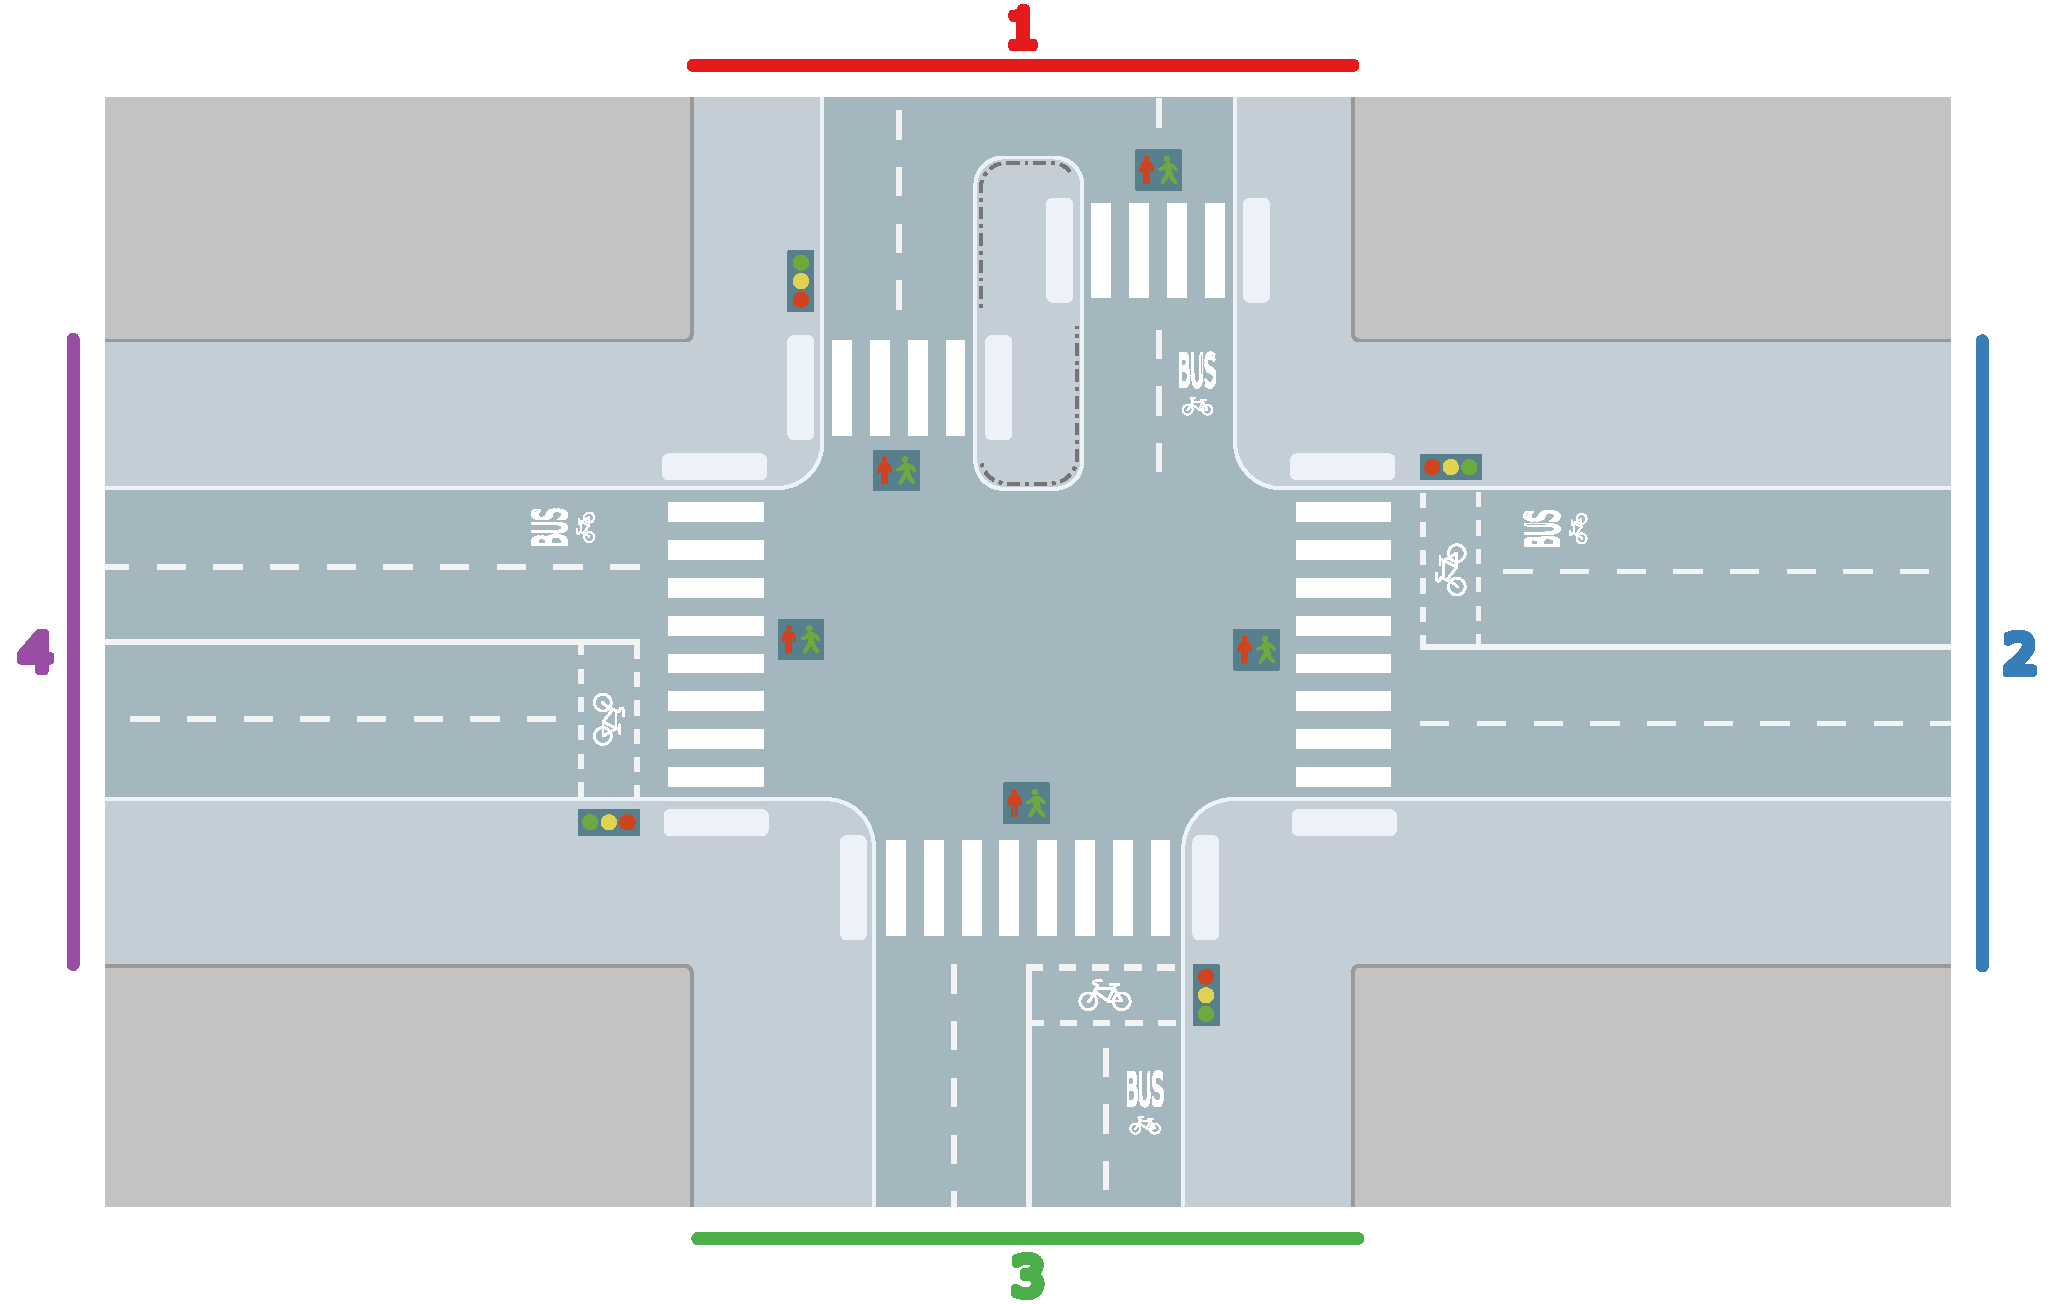
\includegraphics{images/modelisation/mod_branches.pdf}}
    \caption{Ce carrefour composé de quatre branches est dit "en croix".}
    \label{fig:modelisation_branche}
\end{figure}

% Une traversée du carrefour
\begin{figure}
    \centering
    \resizebox{15cm}{!}{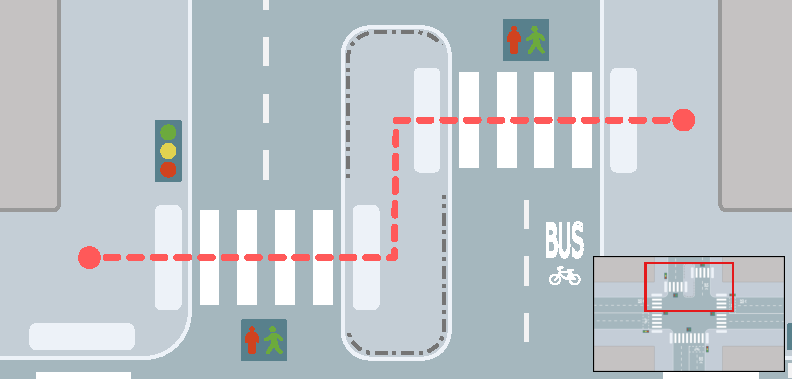
\includegraphics{images/modelisation/mod_traversee.pdf}}
    \caption{Traversée de la première branche du carrefour.}
    \label{fig:modelisation_traversee}
\end{figure}

\todo{}

\subsection{Les repères au sein du carrefour}

\begin{table}
    \begin{center}
    \scriptsize
    \begin{tabular}{ c | m{3cm} | m{10cm} }
        Référence & Image & Description \tabularnewline
        \hline
        1 & \resizebox{3cm}{!}{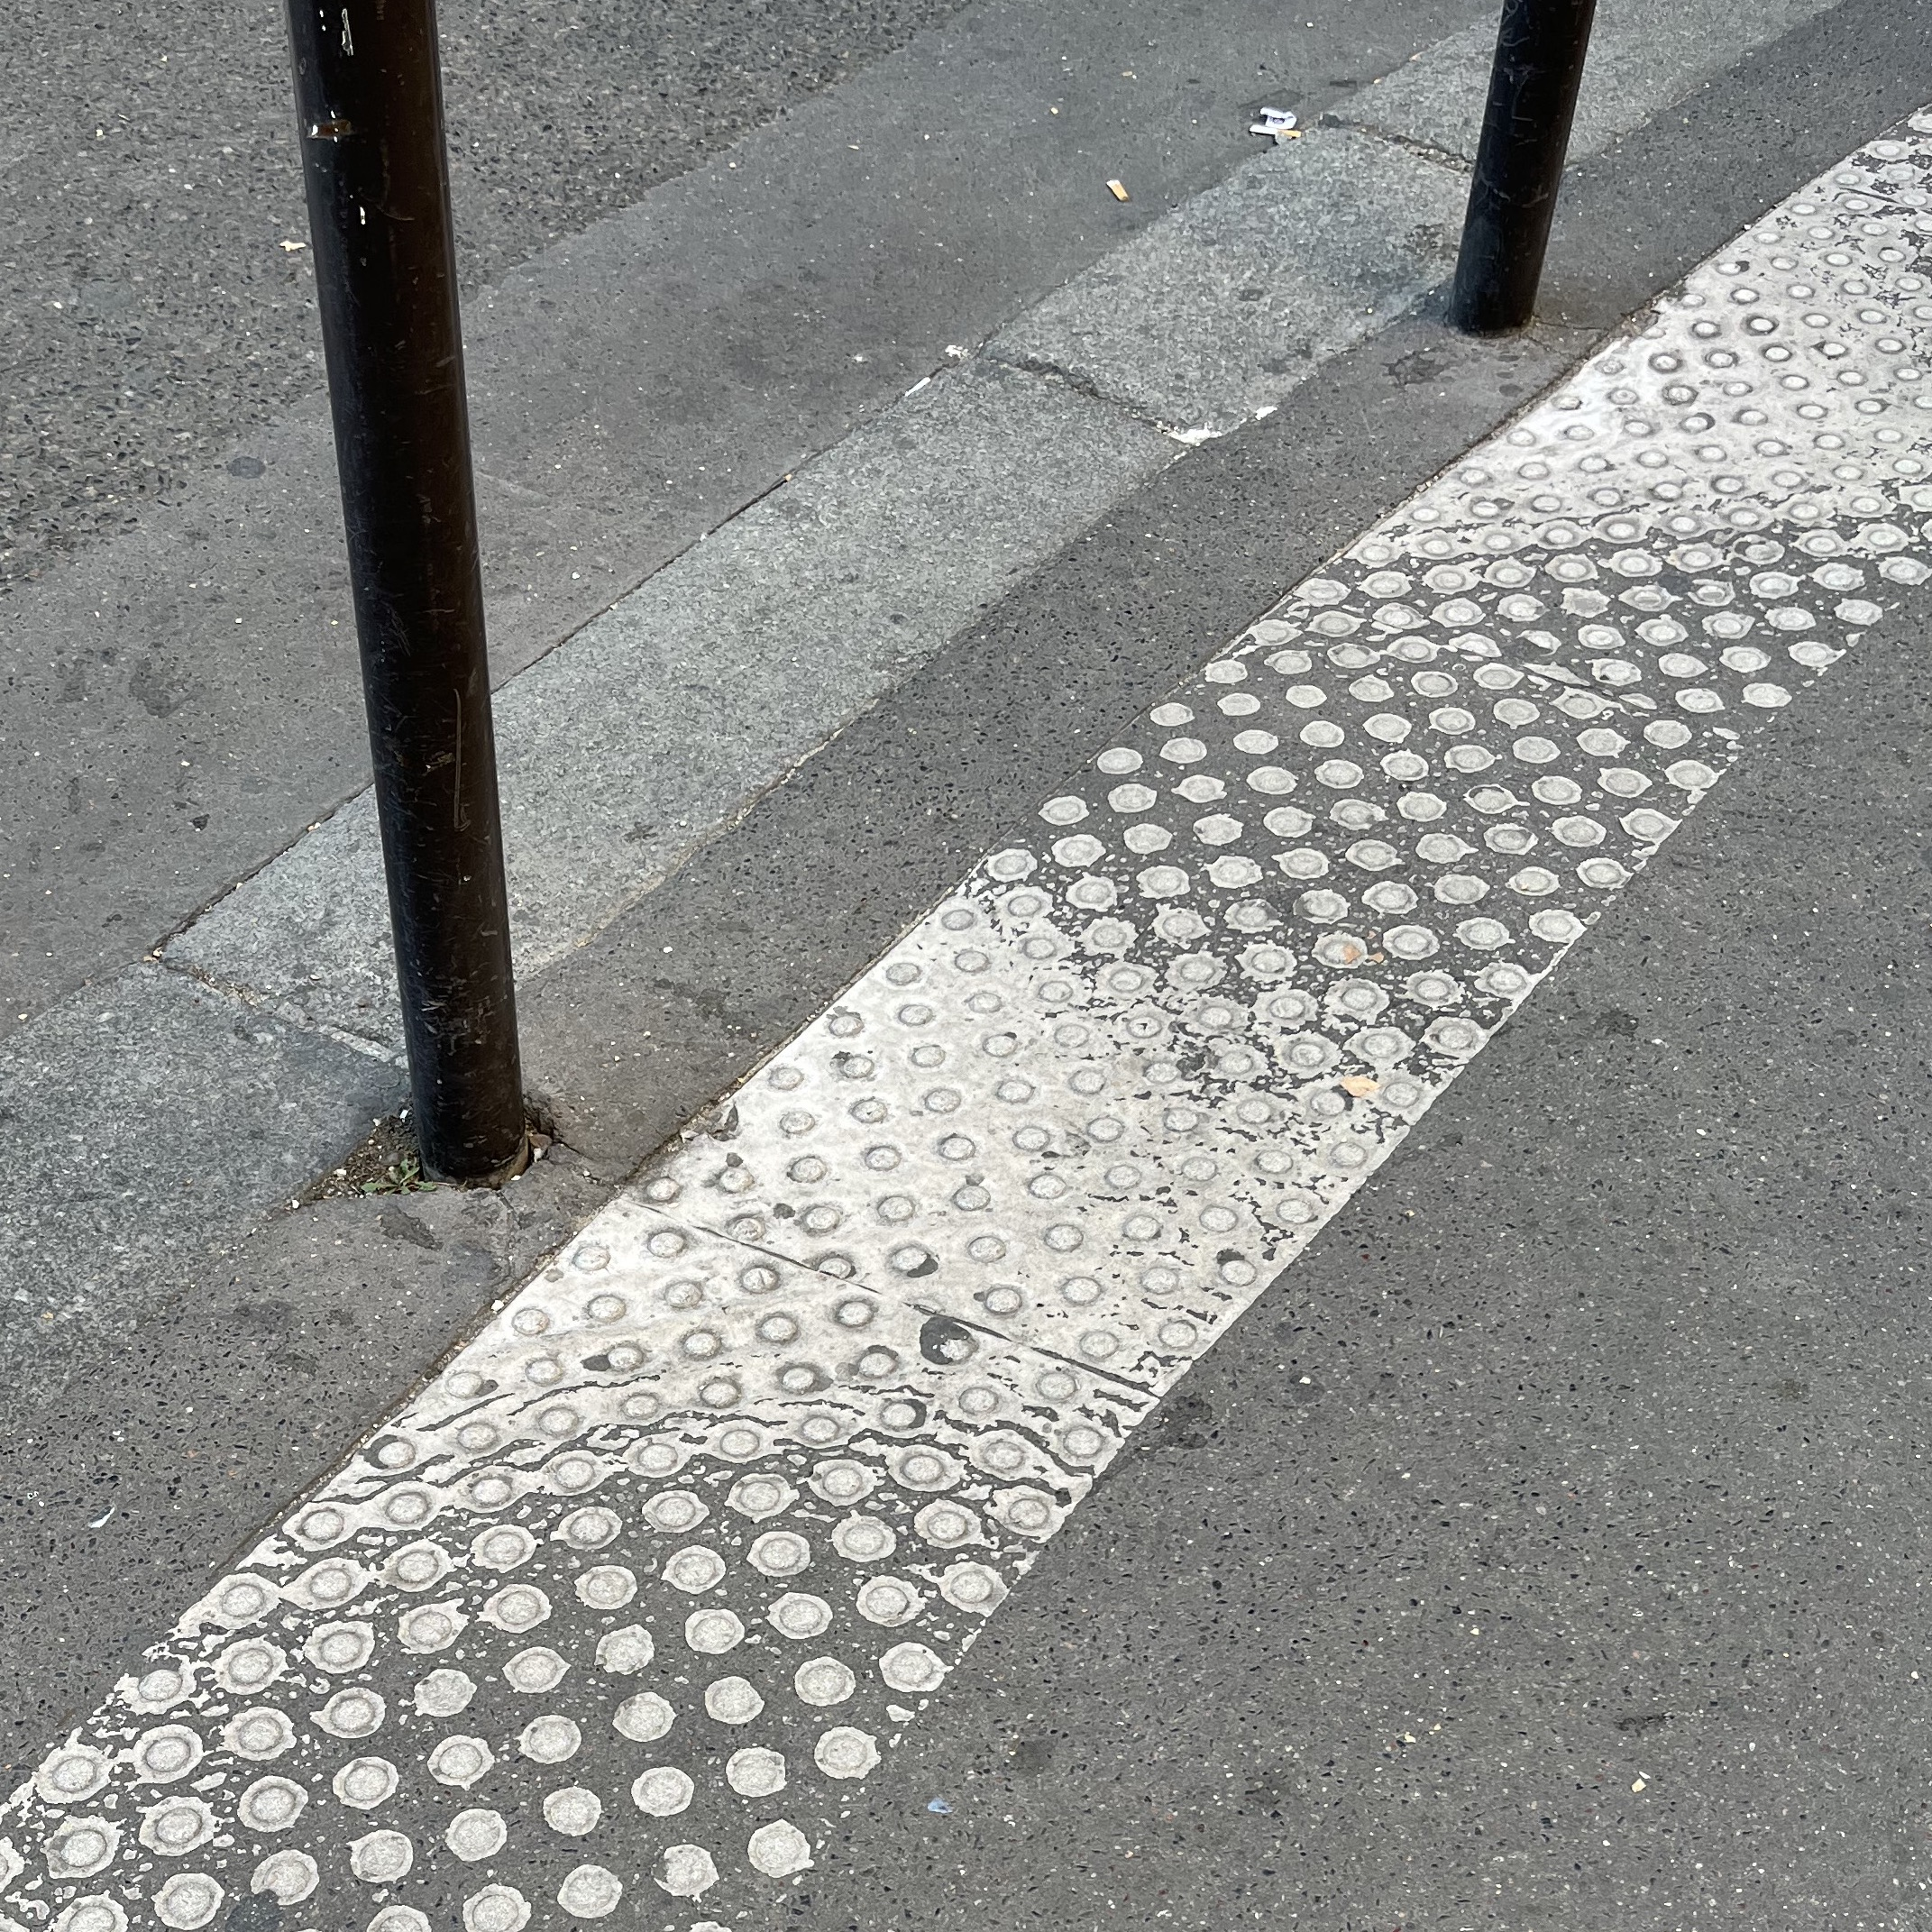
\includegraphics{images/modelisation/mod_bev.jpeg}} & Une \gls{bev} permet de détecter au pied ou à la canne la présence d'un passage piéton. On remarque sur l'image ci-contre qu'elle est abîmée, ce qui peut altérer sa détectabilité.\tabularnewline
        2 & \resizebox{3cm}{!}{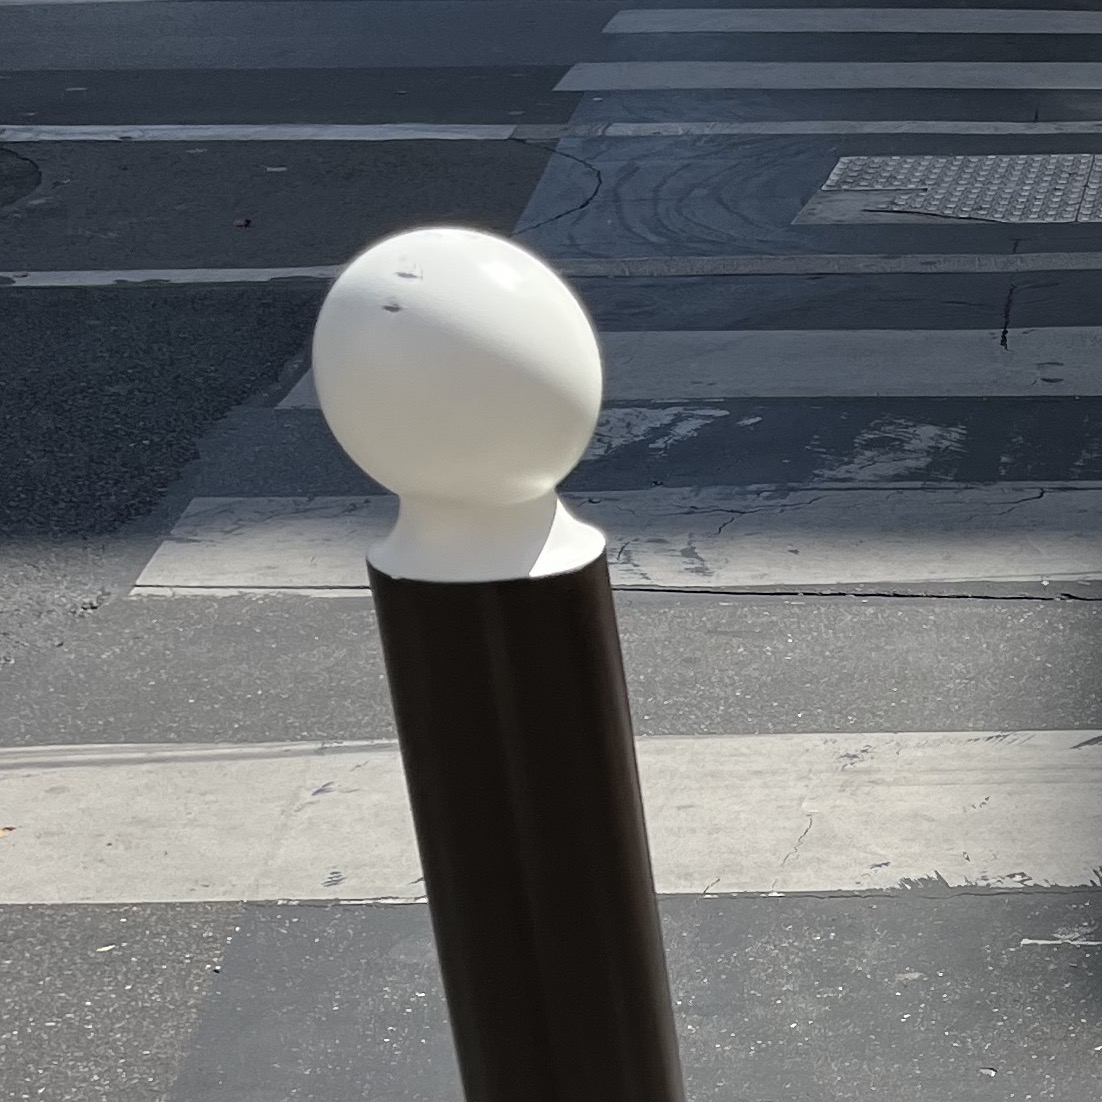
\includegraphics{images/modelisation/mod_poteau.jpeg}} & Les pôteaux parfois présents aux abords des passages piétons permettent à l'inster des \gls{bev} de signaler leur présence. Leur sommet est contrasté avec le corps pour permettre à une personne malvoyante de les distinguer.\tabularnewline
        3 & \resizebox{3cm}{!}{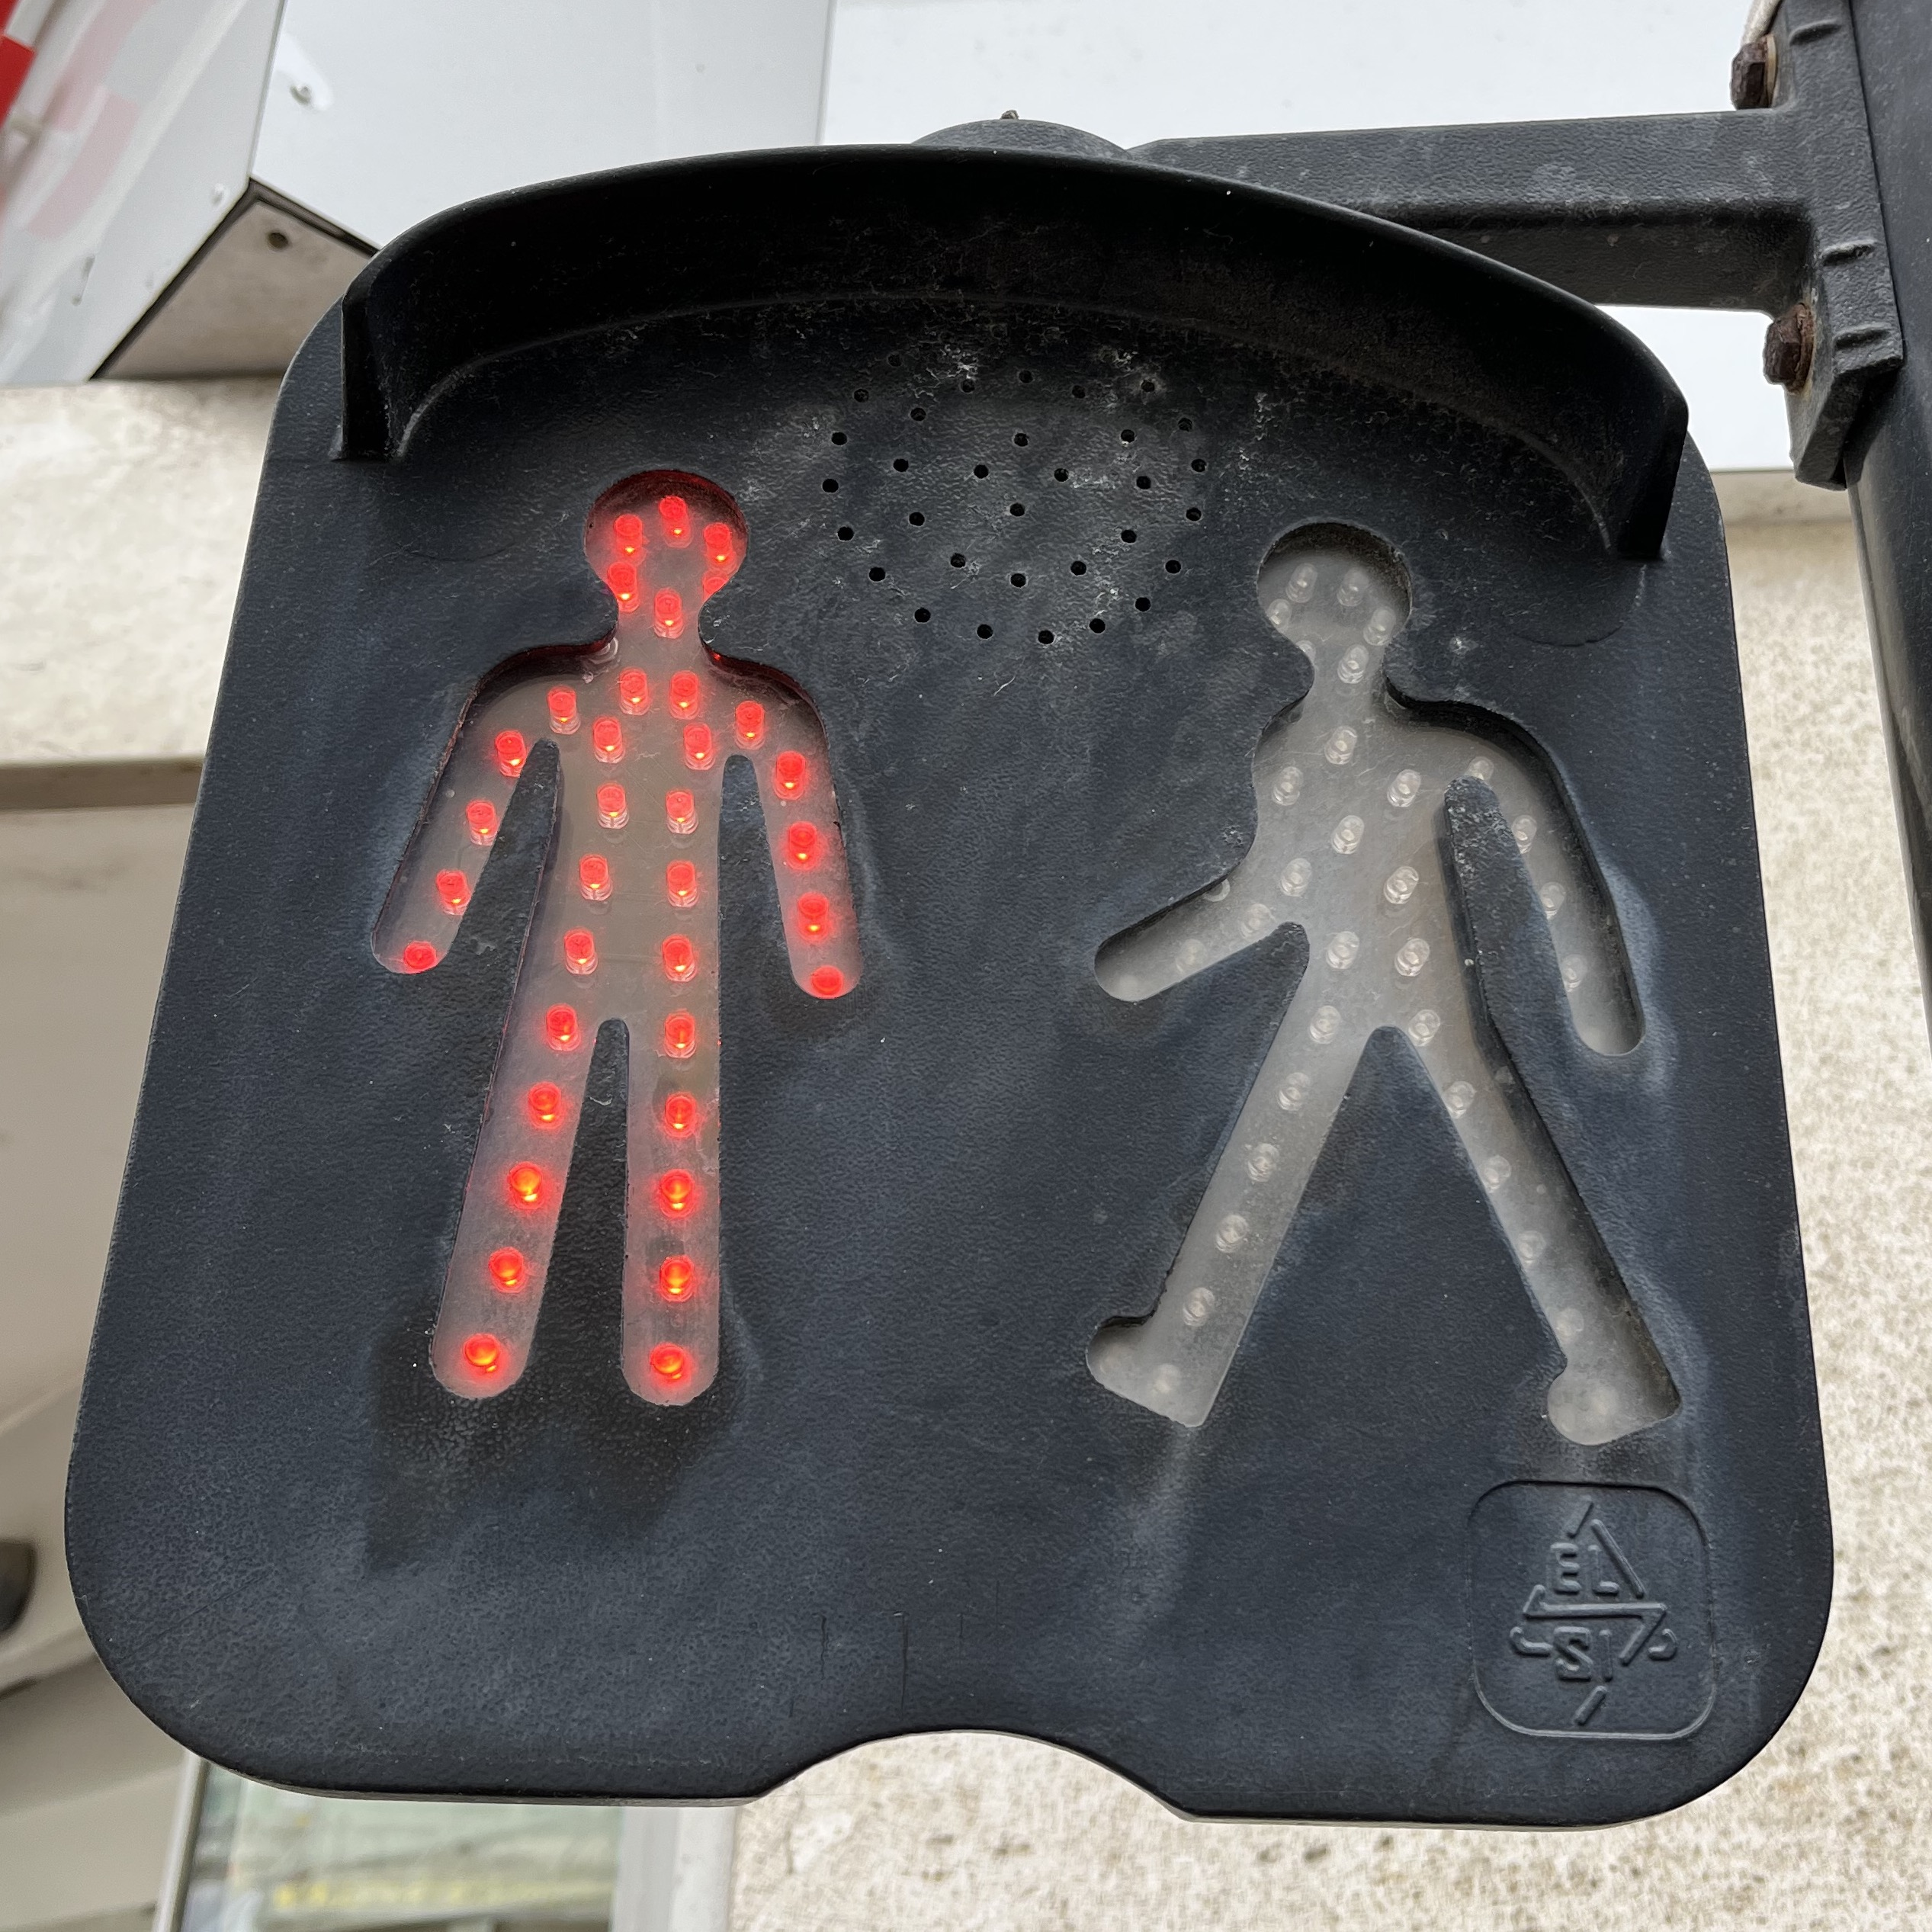
\includegraphics{images/modelisation/mod_feu_pieton.jpeg}} & Les feux de signalisation piéton peuvent être équipés d'une balise sonore. Le message joué par celle-ci varie, mais peut indiquer le nom de la rue traversée lorsque le feu est rouge. Un son de cloche est émis lorsque le feu est vert.\tabularnewline
    \end{tabular}
    \end{center}
    \caption{Équipements d'accessibilité au sein du carrefour.}
    \label{tab:modelisation_objets}
\end{table}

% PCF, obstacles

\todo{}

\section{La modélisation d’un carrefour au sein d’OpenStreetMap}

% En miroir de la partie précédente.
% La délimitation des carrefours n'existe pas dans OSM.
% Celle des branches non-plus.

\gls{osm} est une base de données géographique libre sous licence ODbL. Elle est surtout collaborative et permet à chacun après inscription de contribuer à la cartographie. Nous verrons dans cette partie que, si elle n'est pas particulièrement spécialisée pour la modélisation des carrefours, ses capacités de représentation et la couverture actuelle de certaines données la rendent intéressante pour notre cas d'utilisation.

\subsection{Une forte capacité de représentation}

Plus qu'une base de données géographique, \gls{osm} est une base de données topologique\comment{Ajouter une citation}. Elle permet de représenter 3 types d'objets : les nœuds (node), les lignes (way), et les relations, chacun pouvant contenir une sémantique sous la forme de clés et de valeurs. Les deux premiers sont liés les uns aux autres pour former un graphe. Une route, qui peut apparaître comme une polyligne, est ainsi composée de plusieurs lignes reliées entre elles par des nœuds. 

% Ce que ne permet pas OpenStreetMap

La représentation des carrefours sur OpenStreetMap est en partie possible, mais ne correspond pas entièrement à notre besoin. Il existe la clé junction, qui permet de pointer un carrefour voire de le délimiter (Figure \ref{fig:modelisation_carrefours_osm_paris}). Elle permet, au-delà de la valeur "yes" qui signifie que l'objet concerné est un carrefour, d'indiquer certains types de carrefour, en particulier les ronds-points avec la valeur "roundabout"\footnote{https://wiki.openstreetmap.org/wiki/Key:junction}. Cependant, la sémantique actuelle ne permet pas de modéliser les branches associées au carrefour. Par ailleurs, la plupart des carrefours ne sont pas représentés de cette manière.

\begin{figure}
    \centering
    \resizebox{15cm}{!}{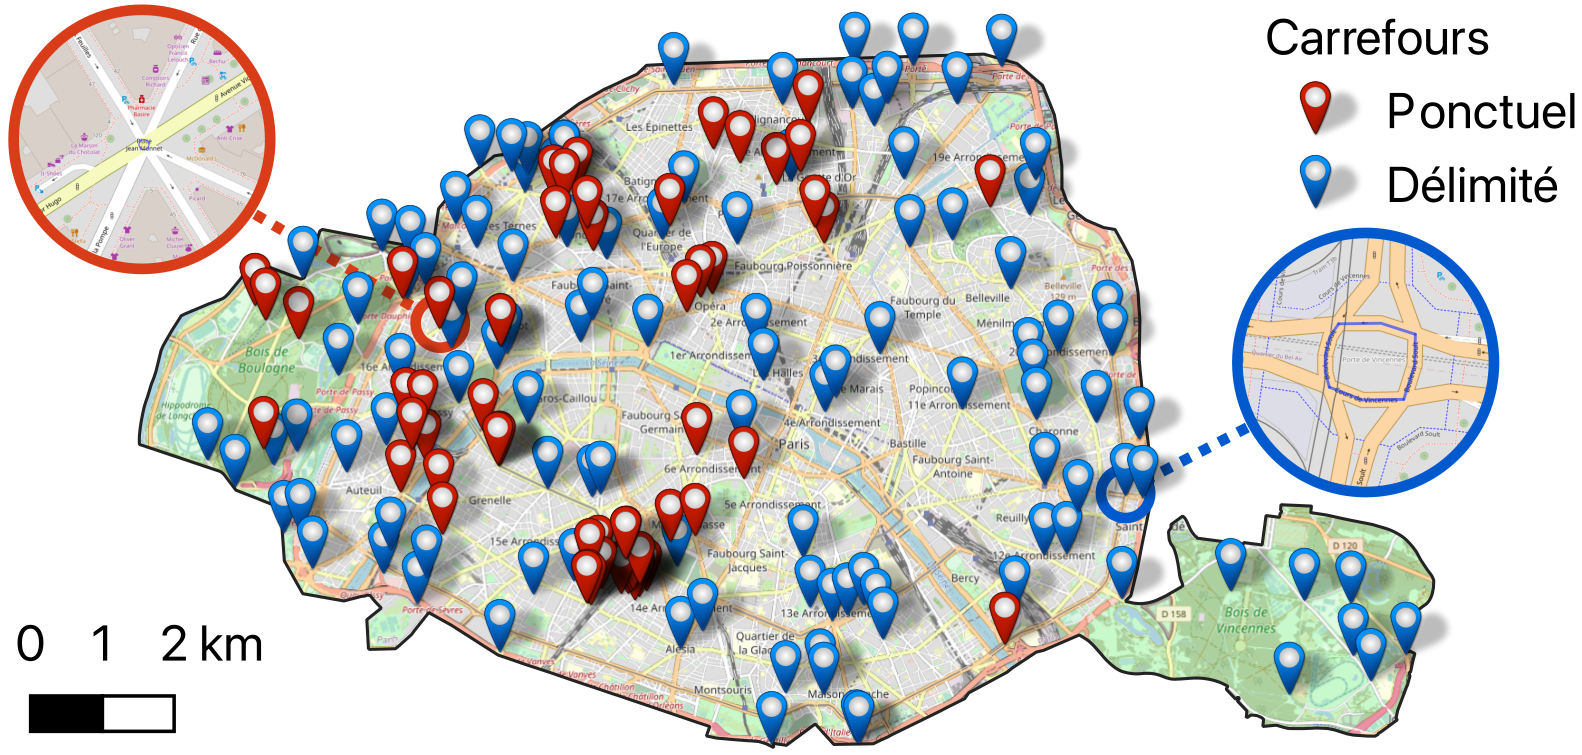
\includegraphics{images/modelisation/mod_carrefours_osm_paris.png}}
    \caption[Les carrefours OSM à Paris.]{À Paris, bien qu'il y ait beaucoup d'objets portant la clé junction, la majorité des carrefours ne sont pas représentés sous cette forme. Source : Contributeurs OpenStreetMap.}
    \label{fig:modelisation_carrefours_osm_paris}
\end{figure}

% Ce que permet OpenStreetMap

En revanche, OpenStreetMap est très souple concernant la représentation de l'accessibilité piétonne, et permet de cartographier finement certains aménagements. Comme le montre la Figure \ref{fig:modelisation_anatomie_carrefour_osm},il est possible d'obtenir un graphe piéton navigable où sont présents les trottoirs et les passages piéton. Les 

\begin{figure}
    \centering
    \resizebox{15cm}{!}{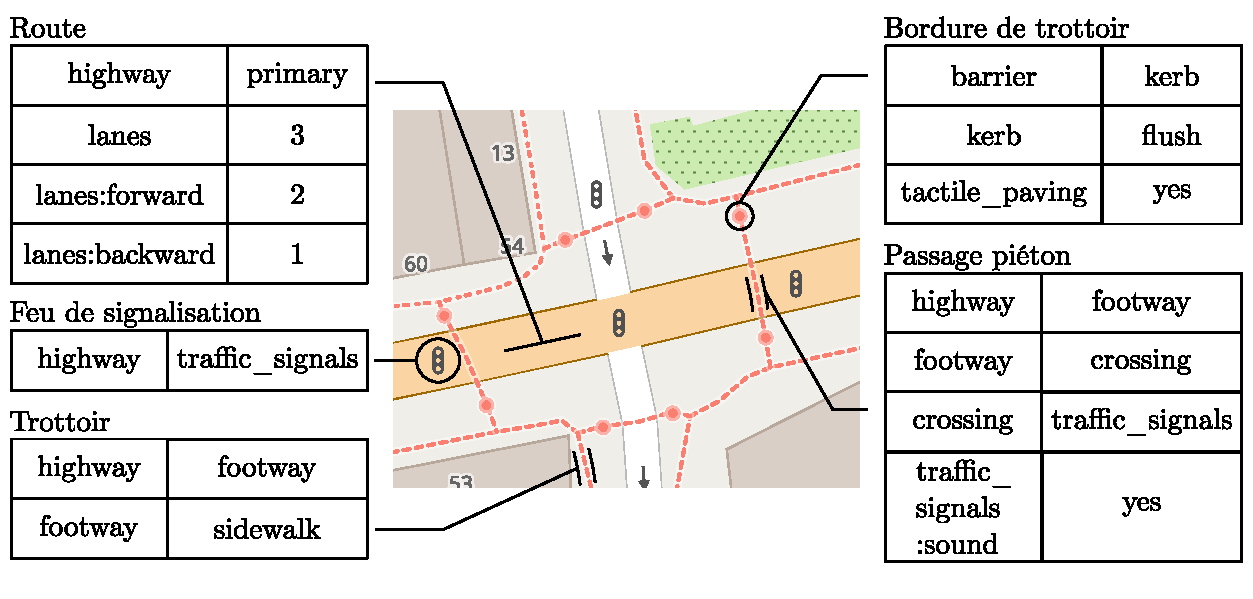
\includegraphics{images/modelisation/mod_anatomie_carrefour_osm.pdf}}
    \caption[Anatomie d'un carrefour dans OSM.]{Exemple de carrefour et des attributs associés dans OpenStreetMap. Outre le graphe piéton, des indications sur l'équipement d'accessibilité ou la largeur des voies sont également présentes. Source : Contributeurs OpenStreetMap.}
    \label{fig:modelisation_anatomie_carrefour_osm}
\end{figure}

\todo{}

\subsection{Des variations dans les modélisations}

% Variation dans la modélisation des trottoirs
% Variation dans la modélisation d'un passage piéton
% Etc.

\todo{}

\section{Un modèle de carrefour}

Pour utiliser la donnée \gls{osm} dans un contexte spécifique, il est préconisé de la manipuler à l'aide d'un modèle de donnée spécialisé intermédiaire \cite{Touya2014}. Nous proposons dans un premier temps une modélisation objet générique de la donnée \gls{osm}, que nous appliquons dans un second temps à la modélisation du carrefour. Enfin, nous présentons les méthodes permettant d'instancier ce modèle depuis OpenStreetMap.

\subsection{OSM-Objet : une modélisation objet de la donnée OpenStreetMap}

\todo{}

\subsection{Application à la modélisation du carrefour}

\todo{}

\subsection{Instancier le modèle depuis OpenStreetMap}

\todo{}